% Designed Companion Part IV figure
% Intended for \input{...} beside the matching canonical problem.
\begin{figure}[ht]
\centering
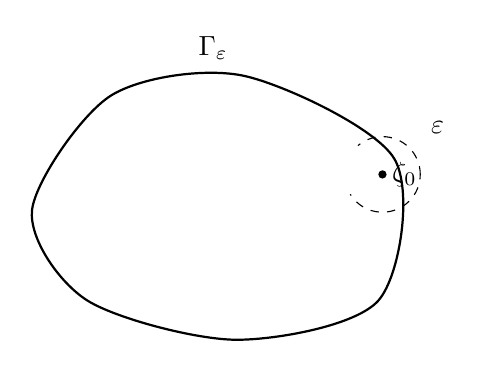
\begin{tikzpicture}[scale=1.0]
  \draw[thick] plot[smooth cycle] coordinates {(-2.4,0) (-1.4,1.45) (0.3,1.7) (2.2,0.65) (2,-1.15) (0.2,-1.65) (-1.7,-1.15)};
  \fill (2.05,0.45) circle (1.5pt) node[right] {$\zeta_0$};
  \draw[dashed] (2.05,0.45) circle (0.48);
  \draw[white,line width=5pt] (1.72,0.83) arc[start angle=135,end angle=215,radius=0.48];
  \node at (2.75,1.05) {$\varepsilon$};
  \node at (-0.1,2.05) {$\Gamma_\varepsilon$};
\end{tikzpicture}
\caption{The principal value contour $\Gamma_\varepsilon$ is obtained by deleting the small arc of $\Gamma$ inside the $\varepsilon$-disk about the singular boundary point $\zeta_0$ and then letting $\varepsilon\downarrow0$.}
\label{fig:cp-iv-0015-principal-value-deleted-arc}
\end{figure}
